\documentclass[a4paper,11pt]{article}
\usepackage[utf8]{inputenc}
\usepackage[T1]{fontenc}
\usepackage[french]{babel}
\usepackage[right=2.5cm, left=2.5cm, bottom=4cm, top=3cm]{geometry}
\usepackage{textcomp}
\usepackage{graphicx}
\usepackage{mathtools,amssymb,amsthm}
\usepackage{lmodern}
\usepackage{array}


\title{\vspace{13em}{\huge Cahier des Charges}}
\author{Edouard Fouassier - Maxime Gonthier - Benjamin Guillot\\
		Laureline Martin - Rémi Navarro - Lydia Rodrigez de la Nava
		\vspace{2em}\\
		Algorithme Genetique
		\vspace{2em}}

\begin{document}
	
	\pagenumbering{gobble}\clearpage
	\maketitle\vspace{13em}
\newpage
\tableofcontents
\newpage\clearpage\pagenumbering{arabic}
	
	\section*{Introduction}
		Le nom algorithme génétique vient des ressemblances avec le monde du vivant, il y a en effet des mutations, des générations et de la sélection naturelles pour n’en citer que quelques un. 
		Cet algorithme a été étudié par John Holland de 1960 à 1975 dans son ouvrage Adaptation in Natural and Artificial System inspiré entre autres par la “learning machine” de Turing.\\
		\\
		L’algorithme génétique s’applique à une grande variété de domaines. 
		Tout d’abord, il peut s’appliquer en génétique pour étudier l’évolution des gènes d’une espèce donnée sur plusieurs générations. 
		On peut aussi appliquer l’algorithme dans le cas d’apprentissage comme par exemple apprendre à un robot à se déplacer en fonction des obstacles. 
		Un troisième domaine d’application possible est l’optimisation. 
		On peut citer dans cette catégorie l’optimisation de portefeuille d'action en fonction de leurs risques ou bien l’optimisation de la ventilation dans le cas de feu dans des espaces confinées ou bien simplement l’optimisation d’une fonction.\\ 
		\\
		L’algorithme génétique est particulièrement utile lorsque l’utilisateur étudie une population et qu’il recherche une solution approchée parmi ces valeurs. 
		Les algorithmes génétiques se démarquent des autres car ils sont très facilement adaptables à différents problèmes. 
		On utilise des règles de transition probabiliste, ce qui est pertinent pour des problèmes où les résultats sont des valeurs approchées.\\

	\section{Fondement du projet}
		\subsection{But du projet}
			L'objectif du projet est de réaliser un programme utilisant un algorithme génétique permettant de délivrer une solution ou un ensemble de solutions optimale(s) d’un problème donné à l’utilisateur en fichier de sortie.
		
		\subsection{Personnes et organismes impliqués dans les enjeux du projet}
			Le projet a pour client principal madame Leila Kloul.
			
		\subsection{ Utilisateurs du produit}
			Le produit se veut se veut employable par n’importe qui cherchant une réponse adaptée à un problème d’optimisation lié à une fonction.
			
	\section{Contraintes sur le projet}
		\subsection{Contraintes non négociables}
			Le logiciel doit permettre à l’utilisateur d’entrer les données de son problème dans une interface textuelle ou en sélectionnant un fichier texte contenant déjà celles-ci.
			De plus, l’algorithme génétique doit être générique afin de fournir une utilisation indépendante du problème à traiter. 
			Enfin, l’utilisateur doit pouvoir obtenir en sortie un fichier montrant l’évolution de l’algorithme durant l’opération.
			Il doit pouvoir choisir entre les formats suivants : Xfig et/ou  LaTeX et/ou PostScript.
		
		\subsection{Glossaire et conventions de dénomination}
			Nous utiliserons dans la suite du cahier des charges les termes suivants pour parler de l’algorithme génétique :\\
			\begin{itemize}
			\item Une \textbf{population d’individu} est un ensemble de solutions potentielles. C’est l’ensemble de données sur lequel l’application sera utilisée afin d’en tirer le meilleur résultat possible.
			\item Un \textbf{individu} ou un \textbf{chromosome} est une solution potentielle au problème donné.
			\item La \textbf{taille} d’un individu s’exprime en puissance de 2. C’est la taille de la solution potentielle au problème (elle peut s’exprimer sous la forme d’un tableau, d’une chaîne,...).
			\item Un \textbf{gène}  est une partie de solution.
			\item L’\textbf{alphabet} est l’ensemble de caractères composant une solution (ex : {0,1} si on utilise des solutions codées en binaire)
			\item Une \textbf{génération } est une itération de l’algorithme génétique utilisé dans l’application. Elle correspond à une modification de l’ensemble de solution. 
			\item La \textbf{fonction fitness} est la fonction que l’on cherche à optimiser dans l’application. Elle servira également à évaluer la qualité des solutions de l’ensemble.
			\item La \textbf{reproduction} correspond à la sélection de solutions de l’ensemble de base afin de les utiliser pour former de nouvelles solutions potentielles.
			\item La \textbf{Mutation} correspond à une modification ponctuelle d’une solution.
			\item Le \textbf{crossover} est le croisement de solutions utilisé pour en créer de nouvelles.
			\end{itemize}
			
		\subsection{Faits et hypothèses utiles}
			Il est impossible de produire un programme totalement générique, c’est pourquoi nous limitons ici l’utilisation du logiciel aux problèmes d’optimisation et de prédiction. 
			Pour l’utiliser dans des problèmes d’apprentissage, il faudrait le coupler avec un autre programme comme un système de classifieur, ou encore un réseau de neurone, ce qui n’est pas le cas dans ce projet.
	\section{Exigences fonctionnelles}
		\subsection{Portée du produit}
		
		\subsection{Exigences fonctionnelles et exigences sur les données}
			
			
	\section{Exigences non fonctionnelles}
		\subsection{Ergonomie et convivialité du produit}
			Le produit devra avoir une interface intuitive et lisible pour faciliter son utilisation et les fichiers de sortie devront être simple à comprendre.
		
		\subsection{Facilité d’utilisation et facteurs humains}
			L’utilisation du logiciel ne doit nécessiter aucun pré-requis à l’utilisateur autre que la connaissance du problème auquel il cherche une solution. 
			Le logiciel doit ainsi procéder à une vérification de tous les champs remplis.
		
		\subsection{Maintenance, support, portabilité, installation du produit}
			L'installation du logiciel devra être simple.\\
			L'ajout ou la modification de module ne devra pas necessiter un de gros changement.\\
			Le produit ne sera dans un premier temps developper que pour linux.\\
			
	\section{Organigramme}
		\centerline{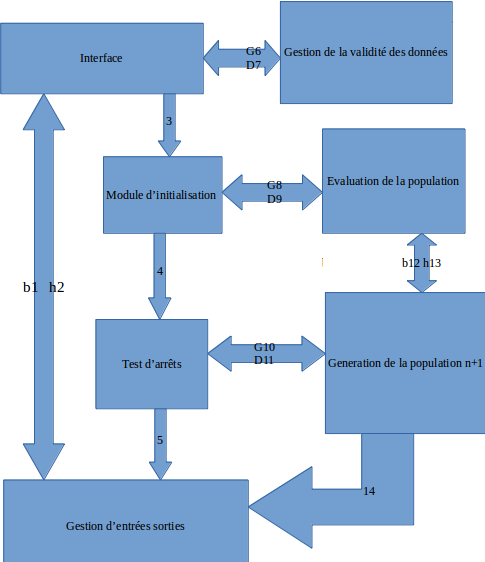
\includegraphics[width = 12cm,height = 10cm]{OrganigrammeV2.png}}
		\begin{center}
			\begin{tabular}{|l l|}
				\hline
				1. Fichier & 8. Population\\
				2. Fichier & 9. Population + score\\
				3. Données initiales & 10. Génération de base 1 (pop size, t mutation, t cross over)\\
				4. Génération 0 et Données initiales & 11. Nouvelle génération après regénération (génération n+1)\\
				5. Génération n + nom fichier & 12. Population\\
				6. Données initiales & 13. Population + score\\
				7. Données initiales & 14. Génération n+1 + nom fichier\\
				\hline 	
			\end{tabular}
		\end{center}
		
		Les données initiales sont :  taux de mutation, Identifiant plus tableau pour le test, fonction fitness, nombre de génération, score à atteindre sur la fonction, taille individu, critère d’évaluation, nombre de critères, alphabet, taille population, probabilité de crossover, nom de fichier.\\
		\\
		\underline{Interface :}
			\begin{itemize}
			\item Affichage
			\end{itemize}
		
		\hspace{1cm}\\
		\underline{Gestion de la validité des données : }
		\begin{itemize}
			\item
		\end{itemize}
		
		\hspace{1cm}\\
		\underline{Module d'initialisation : }
		\begin{itemize}
			\item
		\end{itemize}
	
		\hspace{1cm}\\
		\underline{Evaluation de la population : }
		\begin{itemize}
			\item
		\end{itemize}
		Algorithme Evaluation :
		
		\hspace{1cm}\\
		\underline{Tests d'arrets : }
		\begin{itemize}
			\item
		\end{itemize}

		\hspace{1cm}\\
		\underline{Generation de la population n+1 : }
		\begin{itemize}
			\item
		\end{itemize}
		Algorithme Crossover :
		
		\hspace{1cm}\\
		Algorithme Mutation :
		
		\hspace{1cm}\\
		\underline{Gestion d'entrées sortie : }
		\begin{itemize}
			\item
		\end{itemize}
		
	\section{Autres aspects du projet}
		\subsection{Tâches à faire pour livrer le système}
		
		\subsection{Estimation des coûts du projet}
			\begin{tabular}{|c|c|c|}
				\hline Module & Nombre de lignes & Affectation \\
				\hline 	 &  &  \\
				\hline 	 &  &  \\
				\hline 	 &  &  \\
				\hline 	 &  &  \\
				\hline   &  &  \\
				\hline 	 &  &  \\
				\hline 	 &  &  \\
				\hline 	 &  &  \\
				\hline 	 &  &  \\
				\hline \textbf{Coût Total} & \textbf{XXX} & \textbf{Estimation totale du coût}\\
				\hline 	
				\end{tabular}\vspace{1em}
				
		\subsection{Manuel utilisateur et formations}
		
		\subsection{Idées pour les futures versions}
		
		\subsection{Idées de solutions}
	
	\section{Choix du langage}
	
	\section*{Conclusion}
	
	\section*{Bibliogrophie}
	

\end{document}
